% !TEX root = main.tex
% =====================================================================
% Chapter 8 -- Artificial Intelligence and Data-Driven Estimation
% (SIMPLIFIED + EXPANDED VERSION, matching the treatment applied to
%  Chapter 6: heavy equations replaced with light, intuitive versions;
%  every image slot uses a REAL \includegraphics figure block, not just
%  a comment; content has been lengthened with more explanation,
%  worked examples, and reference tables; tables use \footnotesize and
%  narrow fixed-width columns so nothing overflows the 12.2 cm B5 text
%  column.)
% =====================================================================

\chapter{Artificial Intelligence and Data-Driven Estimation}
\label{ch:ai_data_driven}

\section{Introduction to AI in Battery Systems}
\label{sec:ai_intro}

Traditional parameter estimation algorithms -- such as Recursive Least Squares (RLS), the Extended Kalman Filter (EKF), and the observers covered in Chapter~6 -- all rely on a fairly rigid, hand-built mathematical description of the battery (the equivalent circuit model). This works well in controlled lab conditions, but real batteries are messier than any equivalent circuit: they experience complex multi-physics coupling between heat, chemistry, and mechanical swelling; they see rapid thermal swings during fast charging; and their behavior drifts non-linearly over thousands of cycles as they age. A hand-built model that was accurate on day one may no longer describe the battery well after a year of real-world use.

Artificial Intelligence (AI) and Machine Learning (ML) approaches take a fundamentally different strategy: instead of writing down equations that describe the battery, we let a model \emph{learn} the relationship between what we can measure and what we want to know, directly from historical data. By feeding a model large amounts of recorded current $I(t)$, terminal voltage $V_t(t)$, and cell temperature $T(t)$, the model learns to predict quantities that are otherwise hidden, such as the internal resistance $R_0$, the polarization resistance and capacitance $R_1, C_1$, the remaining usable capacity $C_{\text{cap}}$, or even the entire open-circuit voltage curve $V_{oc}(\text{SOC})$.

\begin{figure}[htbp]
\centering
% Generate this image separately using the prompt below, then save it as:
%   figures/ch8_ai_pipeline.png
% Prompt:
%   "A clean, high-tech vector diagram for a textbook showing an
%    end-to-end data pipeline. On the left, three icons labeled
%    'Voltage', 'Current', and 'Temperature' feed into a box labeled
%    'Feature Extraction (voltage relaxation, ICA peaks, statistical
%    features)'. An arrow leads from that box into a second box
%    labeled 'Machine Learning / Deep Learning Model'. Arrows leave
%    that box toward three output labels: 'SOC', 'SOH', and 'ECM
%    Parameters (R0, R1, C1)'. Flat vector style, blue and grey color
%    palette, white background, clear labeled arrows, no photorealism."
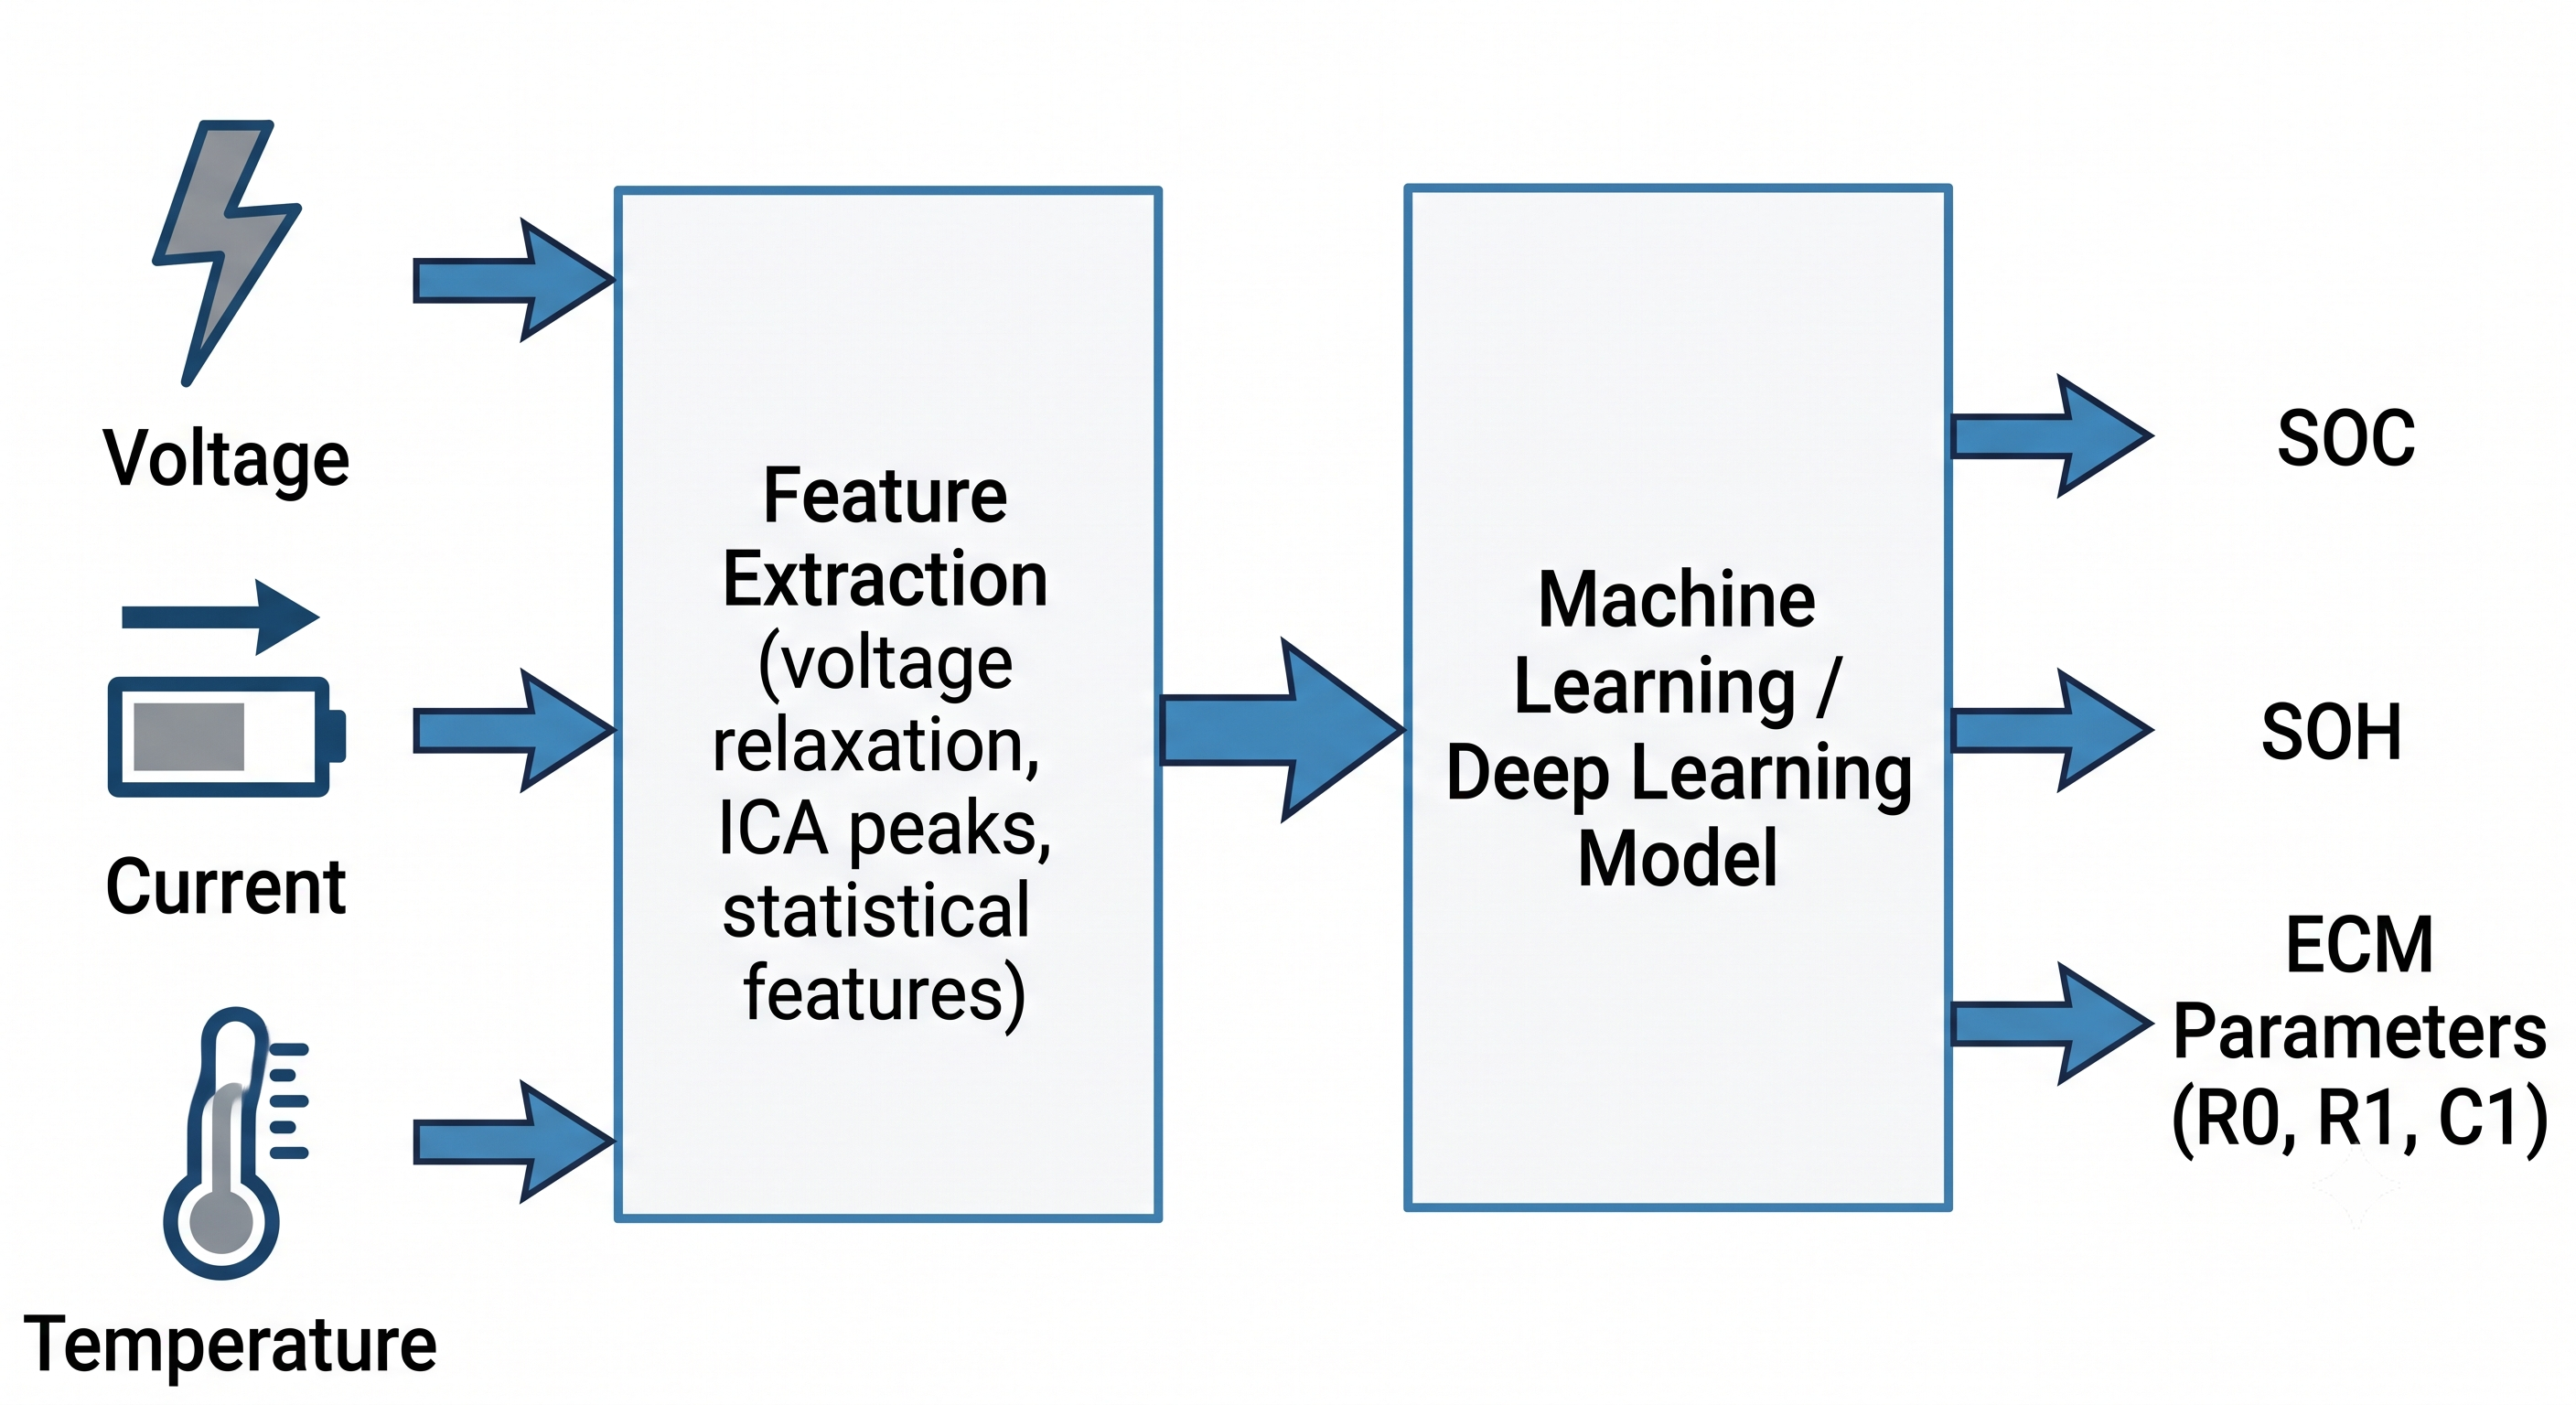
\includegraphics[width=0.9\textwidth]{chp8-1.png}
\caption{End-to-end data-driven BMS estimation pipeline, from raw telemetry to parameter output.}
\label{fig:ch8_ai_pipeline}
\end{figure}

Figure~\ref{fig:ch8_ai_pipeline} shows the general shape of every data-driven estimator discussed in this chapter: raw telemetry is first turned into a handful of informative numbers (feature extraction), and those numbers are fed into a learned model that outputs the parameters we actually care about.

AI-based estimation offers several distinct advantages over the classical approach:
\begin{itemize}
    \item \textbf{Model-Free Non-linear Mapping:} The model learns complex, non-linear relationships between telemetry and parameters automatically, without an engineer needing to derive Jacobian matrices or write closed-form equations by hand.
    \item \textbf{Robustness to Model Mismatch:} Because the model learns directly from real operating data, it naturally captures secondary effects -- voltage hysteresis, SEI (solid-electrolyte interphase) layer growth, electrolyte degradation -- that a simple equivalent circuit model would otherwise miss entirely.
    \item \textbf{Cross-Chemistry Flexibility:} The same overall approach (feature extraction plus a trainable model) can be adapted to a different battery chemistry -- LFP, NMC, or LCO -- simply by retraining on new data, rather than redesigning the whole algorithm from scratch.
\end{itemize}

That flexibility comes with trade-offs, however. Purely data-driven approaches need a curated, representative training dataset; training the model takes computational effort (usually done offline, not on the vehicle); and without extra safeguards, a model can produce physically impossible predictions -- such as a negative resistance -- when it sees operating conditions that were not well represented in its training data. Later in this chapter (Section~\ref{sec:pinns}), we look at one popular way to guard against exactly this problem.

\subsection{Feature Engineering for Battery Telemetry}
Raw current and voltage time-series are rarely fed directly into a machine learning model. Instead, they are first distilled into a smaller set of informative numbers called a \emph{feature vector} $\mathbf{x}$. Good features make the learning task dramatically easier, because they highlight the parts of the signal that actually carry information about battery health, while discarding noise and redundancy. The three most widely used feature families are described below.

\begin{enumerate}
    \item \textbf{Voltage Relaxation Features:} When a load is suddenly disconnected, the terminal voltage jumps almost instantly by an amount $\Delta V_0$, then continues rising more slowly toward its resting value. The instant jump is caused almost entirely by the battery's ohmic resistance, so it gives us a simple, direct estimate:
    \begin{equation}
    R_0 \approx \frac{\Delta V_0}{I_{\text{step}}}
    \label{eq:ch8_r0_estimate}
    \end{equation}
    where $I_{\text{step}}$ is the size of the current step that was removed. The slower part of the relaxation curve -- how long it takes the voltage to settle -- reveals the polarization time constant $\tau_1 = R_1 C_1$: a battery with more internal polarization takes longer to settle after a load step.
    \item \textbf{Incremental Capacity Analysis (ICA):} If we plot how much charge capacity $Q$ changes for a small change in voltage $V$ (written $dQ/dV$), we get a curve with a few clear peaks. These peaks correspond to specific electrochemical reactions happening inside the cell. As a battery ages, these peaks shift position, shrink in height, or merge together -- and those changes correlate directly with how much usable capacity $\Delta C_{\text{cap}}$ the battery has lost.
    \item \textbf{Statistical Features:} Simple statistics computed over a sliding time window -- the mean, variance, skewness, and slope of the voltage relaxation curve -- can pick up subtle changes in internal impedance that build up gradually over hundreds of charge/discharge cycles, even before they become obvious in the raw voltage trace.
\end{enumerate}

Table~\ref{tab:ch8_feature_summary} gives a quick reference for which feature family is best suited to which estimation task, which is a useful starting point when designing a new data-driven estimator.

\begin{table}[htbp]
\centering
\caption{Feature Families and Their Typical Use Cases.}
\label{tab:ch8_feature_summary}
\renewcommand{\arraystretch}{1.3}
\footnotesize
\begin{tabularx}{\textwidth}{|p{2.6cm}|X|p{2.6cm}|}
\hline
\textbf{Feature Family} & \textbf{What It Captures} & \textbf{Best Suited For} \\
\hline
Voltage Relaxation & Instant jump and settling shape after a load step & $R_0$ and $R_1C_1$ tracking \\
\hline
Incremental Capacity (ICA) & Peak position/height in $dQ/dV$ curve & Capacity fade, State of Health (SOH) \\
\hline
Statistical Features & Trend and shape statistics over many cycles & Slow, gradual aging detection \\
\hline
\end{tabularx}
\end{table}


\section{Machine Learning (ML) Methods}
\label{sec:ml_methods}

Once a feature vector $\mathbf{x}$ has been extracted from telemetry, supervised machine learning is used to learn a mapping from $\mathbf{x}$ to a target parameter $y$ (such as $R_0$ or $C_{\text{cap}}$), based on many past examples where both the features and the true parameter value are known.

\subsection{Support Vector Regression (SVR)}
\label{subsec:svr_details}

Support Vector Regression is one of the most widely used "classical" machine learning methods for battery parameter tracking, because it works well with relatively small, clean datasets and rarely needs heavy retraining.

The intuition behind SVR is simple: instead of trying to fit the training points exactly (which would make the model overly sensitive to sensor noise), SVR draws a smooth curve through the data and only worries about points that fall \emph{outside} a small tolerance band around that curve, called the margin $\epsilon$. Any point that falls within the margin is considered "close enough" and is ignored during training, exactly like a deadband. Only the handful of points sitting right at the edge of the margin -- called \emph{support vectors} -- end up shaping the final curve.



In plain terms, the SVR prediction is just a weighted combination of "how similar" a new data point is to each of the support vectors seen during training:
\begin{equation}
f(\mathbf{x}) = \sum_{i=1}^N \alpha_i K(\mathbf{x}_i, \mathbf{x}) + b
\label{eq:ch8_svr_predict}
\end{equation}
where $\alpha_i$ are learned weights, $b$ is a constant offset, and $K(\mathbf{x}_i, \mathbf{x})$ is a similarity score between the new point $\mathbf{x}$ and a training point $\mathbf{x}_i$ -- the more similar two points are, the larger this score. A common and effective choice of similarity score is the Radial Basis Function (RBF), which simply gets smaller the further apart two points are:
\begin{equation}
K(\mathbf{x}_i, \mathbf{x}_j) = \exp\left( -\gamma \|\mathbf{x}_i - \mathbf{x}_j\|^2 \right)
\label{eq:ch8_rbf_kernel}
\end{equation}
Here $\gamma$ controls how "local" the similarity is: a large $\gamma$ means only very nearby points are considered similar (a sharper, more flexible fit), while a small $\gamma$ means the model considers points from further away too (a smoother, less flexible fit).

Table~\ref{tab:ch8_svr_hyperparams} lists recommended SVR hyperparameter configurations for tracking internal resistance $R_0$, along with a plain-language explanation of what each one controls.

\begin{table}[htbp]
\centering
\caption{SVR Hyperparameter Tuning Configurations for $R_0$ Estimation.}
\label{tab:ch8_svr_hyperparams}
\renewcommand{\arraystretch}{1.3}
\footnotesize
\begin{tabularx}{\textwidth}{|p{2.6cm}|c|c|X|}
\hline
\textbf{Hyperparameter} & \textbf{Search Range} & \textbf{Typical Value} & \textbf{Effect on Model} \\
\hline
Regularization $C$ & $10^{-2}$ to $10^4$ & 100 & Trades off a smoother curve against a tighter fit to the data \\
\hline
Margin $\epsilon$ & $10^{-4}$ to $0.1$ & 0.001 & Sets the size of the "ignore small error" deadband \\
\hline
Kernel width $\gamma$ & $10^{-4}$ to $10^{2}$ & 1.0 & Sets how local or global the similarity comparison is \\
\hline
\end{tabularx}
\end{table}

A practical tip: rather than picking these three values by hand, engineers typically run a grid search or random search over the ranges in Table~\ref{tab:ch8_svr_hyperparams}, evaluating each combination on a held-out validation dataset that was not used for training, and keeping whichever combination gives the lowest validation error.

\subsection{Gaussian Process Regression (GPR)}
\label{subsec:gpr_details}

Gaussian Process Regression takes a different, probabilistic approach. Instead of producing just a single predicted number, GPR produces a predicted value \emph{together with} a confidence range around it -- effectively telling you not only "what is $R_0$ probably equal to?" but also "how sure am I about that answer?" This second piece of information is extremely valuable in a safety-critical BMS, because it lets the system distinguish between a confident, trustworthy estimate and a shaky guess made in unfamiliar operating conditions.

In everyday terms, GPR works by comparing a new measurement to every training example it has seen, weighting each comparison by how similar the two situations are (much like the SVR similarity score above). Predictions made close to lots of familiar training data come with a narrow, confident range; predictions made far from any training data -- for example, at an unusually low temperature the model rarely saw during training -- come with a wide, uncertain range. This behavior is summarized compactly as:
\begin{equation}
\hat{y}(\mathbf{x}_*) = \mu_*(\mathbf{x}_*) \pm \sigma_*(\mathbf{x}_*)
\label{eq:ch8_gpr_simple}
\end{equation}
where $\mu_*$ is the predicted value (the model's best guess) and $\sigma_*$ is the predicted uncertainty (how much that guess might be wrong). Both $\mu_*$ and $\sigma_*$ are computed automatically by the GPR algorithm from the training data -- the underlying calculation involves comparing the new input to every training point, but the key idea for a BMS engineer is simply Equation~\eqref{eq:ch8_gpr_simple}: every prediction comes with its own built-in confidence range.

Table~\ref{tab:ch8_gpr_actions} suggests how a BMS might practically react to different levels of GPR-reported uncertainty.

\begin{table}[htbp]
\centering
\caption{Suggested BMS Response to GPR Confidence Levels.}
\label{tab:ch8_gpr_actions}
\renewcommand{\arraystretch}{1.3}
\footnotesize
\begin{tabularx}{\textwidth}{|p{2.6cm}|X|}
\hline
\textbf{Reported Uncertainty $\sigma_*$} & \textbf{Suggested BMS Response} \\
\hline
Low (well within training range) & Use the estimate directly for control decisions. \\
\hline
Moderate & Use the estimate, but flag it for later review or blend it with a fallback model. \\
\hline
High (outside training range) & Mark the estimate as unreliable; revert to conservative power limits or a physics-based fallback model. \\
\hline
\end{tabularx}
\end{table}


\section{Deep Learning for Parameter Extraction}
\label{sec:deep_learning}

Where SVR and GPR both rely on hand-designed features, deep learning models are able to process the raw sequential telemetry stream directly, automatically discovering temporal patterns (such as aging signatures) that might be missed by manually engineered features.

\subsection{Recurrent Neural Networks (LSTM)}
\label{subsec:lstm_details}

A Long Short-Term Memory (LSTM) network is a type of neural network specifically designed to process sequences of data -- such as a time series of current, voltage, and temperature measurements $\mathbf{x}_t = [I_t, V_{t,t}, T_t]^T$ -- while remembering useful information from far earlier in the sequence. This is exactly the kind of memory needed to track slow battery aging: what happened many charge cycles ago still matters for today's prediction.

An LSTM manages its memory using three simple "gates," each of which is easiest to think of as a decision the network makes at every time step:
\begin{itemize}
    \item \textbf{Forget Gate:} Decides which parts of the memory from previous time steps are no longer useful and can be discarded, based on the most recent current and thermal inputs.
    \item \textbf{Input Gate:} Decides which parts of the newest voltage transient information are worth adding into memory.
    \item \textbf{Output Gate:} Uses the current memory contents to produce the network's output at this time step -- the hidden state $\mathbf{h}_t$, which is mapped to the network's parameter estimate $\hat{\boldsymbol{\theta}}_t$.
\end{itemize}
In short: the forget gate cleans out old, irrelevant information; the input gate lets in new, relevant information; and the output gate turns the current memory into a usable prediction.

The network is trained by comparing its predicted parameters $\hat{\boldsymbol{\theta}}_i$ against known true values $\boldsymbol{\theta}_i$ across many training examples, and adjusting the network's internal weights to make that comparison as small as possible on average:
\begin{equation}
\mathcal{L}_{\text{MSE}} = \frac{1}{N} \sum_{i=1}^N \left( \boldsymbol{\theta}_i - \hat{\boldsymbol{\theta}}_i \right)^2
\label{eq:ch8_lstm_loss}
\end{equation}
This is simply the average squared prediction error across all $N$ training examples -- the smaller this number gets during training, the better the network's predictions match reality.

Table~\ref{tab:ch8_lstm_hyperparams} outlines standard hyperparameter configurations for training LSTM parameter estimators on vehicle drive-cycle datasets.

\begin{table}[htbp]
\centering
\caption{Recommended LSTM Architecture Configurations for BMS Parameter Tracking.}
\label{tab:ch8_lstm_hyperparams}
\renewcommand{\arraystretch}{1.3}
\footnotesize
\begin{tabularx}{\textwidth}{|p{3.0cm}|c|X|}
\hline
\textbf{Hyperparameter} & \textbf{Typical Value} & \textbf{Rationale} \\
\hline
Hidden Units & 64--128 & Provides enough capacity to capture non-linear ECM dynamics \\
\hline
LSTM Layers & 2 & One layer for short-term overvoltage behavior, one for long-term thermal trends \\
\hline
Window Length & 100 steps & Long enough to capture a full polarization relaxation cycle \\
\hline
Learning Rate & $10^{-3}$ & A safe default for stable convergence with the Adam optimizer \\
\hline
\end{tabularx}
\end{table}

\subsection{A Worked Comparison: SVR vs. GPR vs. LSTM}
To help decide which method fits a given project, Table~\ref{tab:ch8_method_comparison} compares the three data-driven methods introduced so far across several practical criteria that matter for automotive BMS development.

\begin{table}[htbp]
\centering
\caption{Practical Comparison of SVR, GPR, and LSTM for Parameter Estimation.}
\label{tab:ch8_method_comparison}
\renewcommand{\arraystretch}{1.3}
\footnotesize
\begin{tabularx}{\textwidth}{|p{2.0cm}|X|X|X|}
\hline
\textbf{Criterion} & \textbf{SVR} & \textbf{GPR} & \textbf{LSTM} \\
\hline
Training data needed & Small to medium & Small to medium & Large \\
\hline
Confidence output & No & Yes, built in & Only with extra techniques \\
\hline
Handles raw time series directly & No (needs features) & No (needs features) & Yes \\
\hline
Typical training effort & Low & Low--Medium & High \\
\hline
Best fit for & Well-understood features, limited data & Safety-critical decisions needing confidence bounds & Long, information-rich drive-cycle datasets \\
\hline
\end{tabularx}
\end{table}


\section{Physics-Informed Neural Networks (PINNs)}
\label{sec:pinns}

A purely data-driven neural network has no built-in understanding of physics -- it only knows what it has seen in its training data. When it encounters operating conditions that were poorly represented during training, it can occasionally produce results that are mathematically plausible but physically impossible, such as a negative resistance value or a battery capacity that appears to increase during discharge. Physics-Informed Neural Networks (PINNs) address this weakness by teaching the network the governing physical equations directly, alongside the training data, rather than relying on data alone.



The idea is to give the network three separate goals during training, rather than just one:
\begin{itemize}
    \item Match the measured data as closely as possible.
    \item Obey the known equivalent circuit equations from Chapter~6, as closely as possible.
    \item Stay within physically sensible bounds (for example, resistance and capacitance must always be positive).
\end{itemize}
These three goals are combined into a single training objective:
\begin{equation}
\mathcal{L}_{\text{PINN}} = \mathcal{L}_{\text{data}} + \lambda_{\text{phys}} \mathcal{L}_{\text{physics}} + \lambda_{\text{bound}} \mathcal{L}_{\text{bounds}}
\label{eq:ch8_pinn_loss_total}
\end{equation}
where $\lambda_{\text{phys}}$ and $\lambda_{\text{bound}}$ are simple weighting numbers that control how strongly each goal is enforced relative to the others. Each term is explained below in plain language, with a short representative equation.

\begin{itemize}
    \item \textbf{Data term:} penalizes the difference between the predicted terminal voltage $\hat V_{t,k}$ and the actual measured terminal voltage $V_{t,k}$, averaged over $N$ training samples:
    \begin{equation}
    \mathcal{L}_{\text{data}} = \frac{1}{N} \sum_{k=1}^N \left( V_{t,k} - \hat{V}_{t,k} \right)^2
    \end{equation}
    \item \textbf{Physics term:} penalizes the network whenever its predicted parameters, when plugged back into the ordinary equivalent circuit equation from Chapter~6, would predict a voltage that disagrees with what the network itself predicted:
    \begin{equation}
    \mathcal{L}_{\text{physics}} = \frac{1}{N} \sum_{k=1}^N \left( \hat{V}_{t,k} - V_{\text{ECM},k} \right)^2
    \end{equation}
    where $V_{\text{ECM},k}$ is simply the voltage that the standard equivalent circuit model (open-circuit voltage minus polarization voltage minus ohmic drop) would predict, given the network's own parameter estimates.
    \item \textbf{Bounds term:} a simple penalty that increases sharply if a predicted parameter strays outside its physically valid range, keeping values such as $R_0$ and $C_1$ always positive.
\end{itemize}

By enforcing physical laws during training, PINNs have been shown to reduce the amount of training data needed by up to 70\% compared to a purely data-driven network of the same size, while also guaranteeing that predictions stay within physically sensible bounds -- an important safety property for any estimator that will influence real-time power limits in a vehicle.


\section{Embedded Deployment and Edge AI Considerations}
\label{sec:edge_ai}

A model that performs well on a training server is not automatically ready to run inside a battery management system. Automotive-grade microcontrollers (such as an ARM Cortex-M7 or an Infineon AURIX) have far less memory and computing power than a training server, so trained AI models usually need to be compressed and simplified before deployment.

\begin{enumerate}
    \item \textbf{Quantization:} Model weights are normally stored as 32-bit floating-point numbers during training. Converting them to 8-bit integers (INT8) for deployment shrinks the model's storage footprint by roughly 75\%, with only a small accuracy cost, typically under 0.5\%.
    \item \textbf{Pruning:} Many trained networks contain a large number of weights that are close to zero and contribute almost nothing to the final prediction. Removing these weights reduces the number of multiply-accumulate (MAC) operations the microcontroller must perform at run time, speeding up inference without materially affecting accuracy.
    \item \textbf{Cloud-Edge Co-Processing:} The most computationally expensive part of the whole process -- training a deep learning model on large historical datasets -- is normally done off-board, in the cloud, where memory and compute are effectively unlimited. Only a lightweight, already-trained inference model (such as SVR, GPR, or a quantized/pruned PINN) is deployed onto the vehicle's BMS hardware, where it only needs to make fast predictions, not learn from scratch.
\end{enumerate}

\begin{figure}[H]
\centering
% Generate this image separately using the prompt below, then save it as:
%   figures/ch8_edge_deployment_pipeline.png
% Prompt:
%   "A simple horizontal pipeline diagram for a textbook. Left box
%    labeled 'Cloud: Full-Precision Model Training' connects via an
%    arrow labeled 'Quantization + Pruning' to a middle box labeled
%    'Compressed Model (INT8)'. A second arrow labeled 'Deploy' leads
%    to a right-hand box labeled 'Vehicle BMS Microcontroller:
%    Fast Inference Only'. Flat, clean vector illustration, blue and
%    grey tones, white background, textbook figure style, clear
%    labeled arrows left to right."
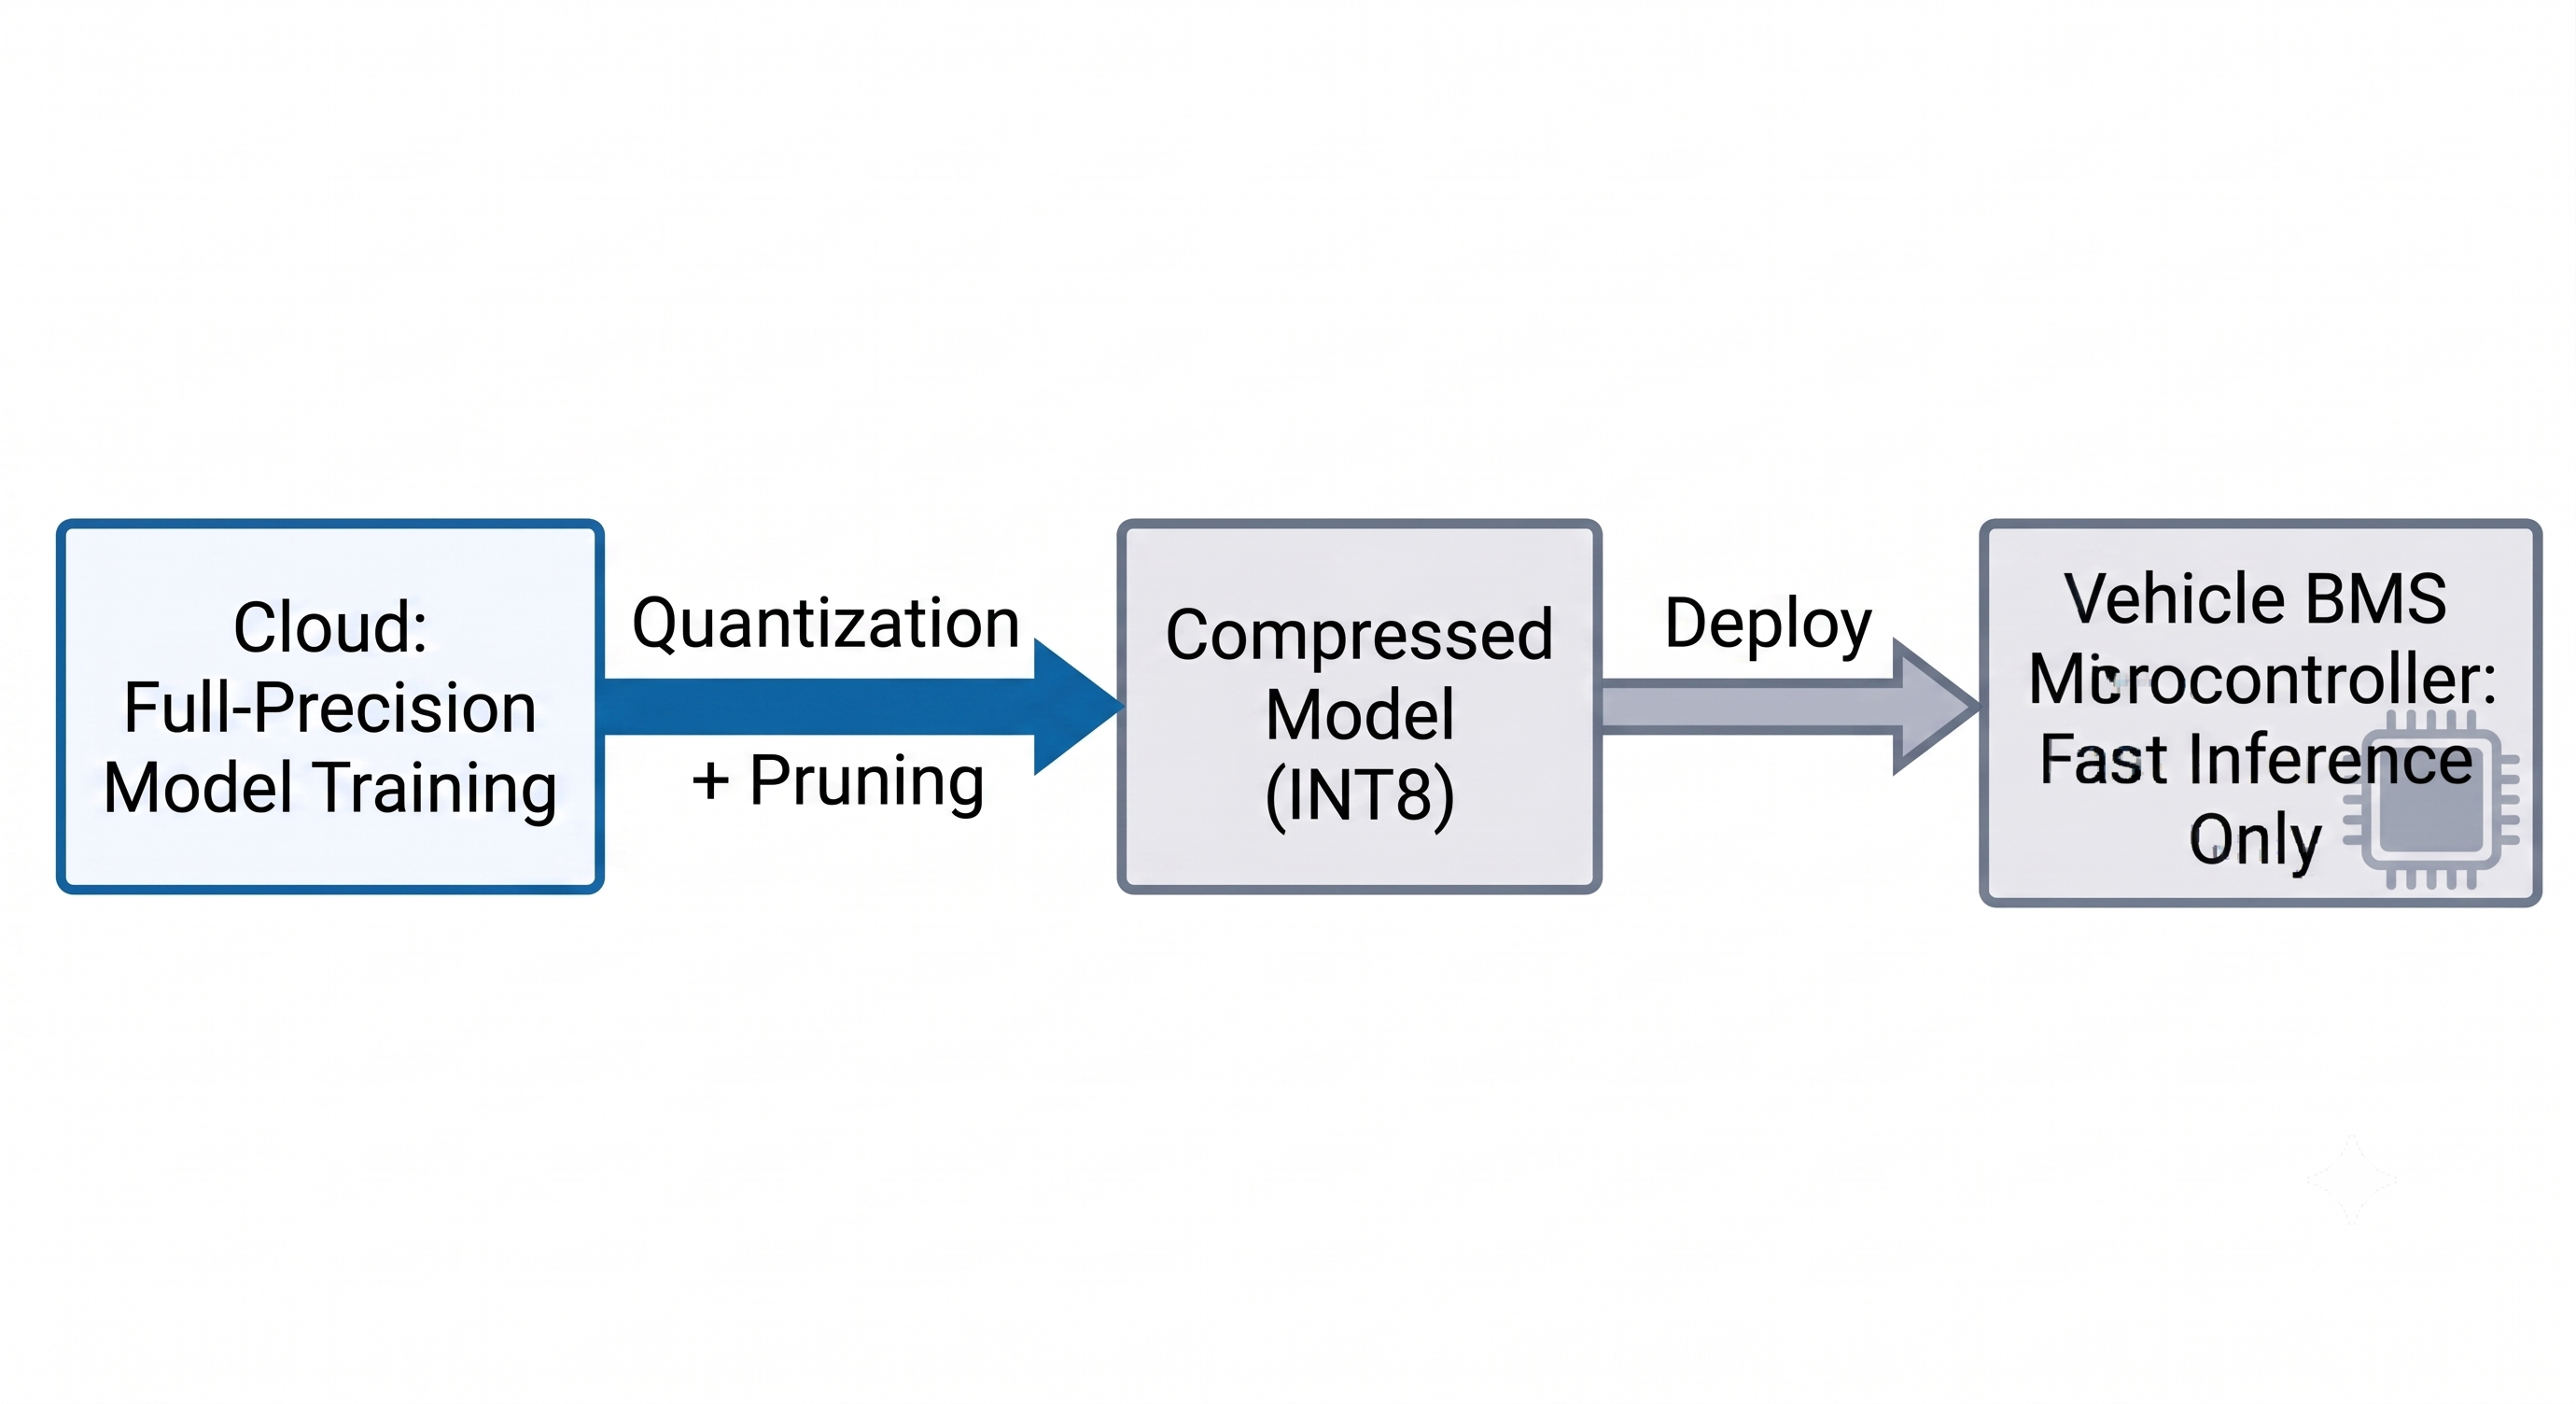
\includegraphics[width=0.9\textwidth]{ch8-4.png}
\caption{Typical cloud-to-edge deployment pipeline: heavy training happens in the cloud, while only a lightweight, compressed model runs on the vehicle.}
\label{fig:ch8_edge_pipeline}
\end{figure}

Table~\ref{tab:ch8_edge_techniques} summarizes when each compression technique is most useful, which is a helpful starting point when deciding how to prepare a trained model for a specific microcontroller's memory and timing budget.

\begin{table}[H]
\centering
\caption{When to Use Each Edge-AI Compression Technique.}
\label{tab:ch8_edge_techniques}
\renewcommand{\arraystretch}{1.3}
\footnotesize
\begin{tabularx}{\textwidth}{|p{2.6cm}|X|}
\hline
\textbf{Technique} & \textbf{Most Useful When...} \\
\hline
Quantization & Storage/flash memory is the tightest constraint. \\
\hline
Pruning & Inference speed (real-time deadline) is the tightest constraint. \\
\hline
Cloud-Edge Co-Processing & The model needs frequent retraining on large, growing datasets. \\
\hline
\end{tabularx}
\end{table}


\section{Choosing the Right Method for a Given Project}
\label{sec:ch8_choosing_method}

With four broad families of data-driven methods now introduced -- SVR, GPR, LSTM, and PINNs -- it is worth stepping back and asking a practical question: which one should be used for a new project? There is no single correct answer, but a few simple rules of thumb, summarized in Table~\ref{tab:ch8_decision_guide}, cover most real-world situations.

\begin{table}[htbp]
\centering
\caption{Simple Decision Guide for Selecting a Data-Driven Estimation Method.}
\label{tab:ch8_decision_guide}
\renewcommand{\arraystretch}{1.3}
\footnotesize
\begin{tabularx}{\textwidth}{|X|p{3.2cm}|}
\hline
\textbf{If your project has this priority...} & \textbf{...then start with:} \\
\hline
Small dataset, limited engineering time & SVR with hand-designed features \\
\hline
Safety-critical decisions that need a confidence estimate & GPR \\
\hline
Large, information-rich drive-cycle datasets and enough compute budget & LSTM \\
\hline
Limited training data but strong need for physically valid predictions & PINN \\
\hline
Tight microcontroller memory or timing budget & Whichever method above fits, then apply quantization and pruning from Section~\ref{sec:edge_ai} \\
\hline
\end{tabularx}
\end{table}

In practice, many production battery management systems do not rely on a single method in isolation. A common and pragmatic architecture is to run a lightweight classical estimator (such as the observers from Chapter~6, or an SVR model) as the primary, always-on estimator, while a more powerful but occasional deep learning or PINN model runs periodically -- for example, once per charging session -- to recalibrate the lightweight estimator's parameters. This hybrid approach captures much of the accuracy benefit of deep learning while keeping the real-time computational burden on the vehicle's microcontroller low.


\section{Chapter Summary}
\label{sec:ch8_summary}

Data-driven machine learning and physics-informed neural networks complement the classical estimation methods covered earlier in this book, rather than replacing them outright. By combining thoughtful feature extraction (Section~\ref{sec:ai_intro}) with either classical learning methods (SVR, GPR) or deep sequence models (LSTM), and by optionally constraining predictions with known physics (PINNs), AI-based estimators can provide robust parameter tracking across diverse lithium-ion chemistries and demanding, real-world operating conditions.

The key practical takeaways from this chapter are:
\begin{itemize}
    \item Good features (voltage relaxation, incremental capacity, and simple statistics) often matter as much as the choice of learning algorithm itself.
    \item SVR and GPR are strong, low-effort starting points for smaller datasets, with GPR offering the added benefit of a built-in confidence estimate.
    \item LSTM networks unlock the most accuracy when a large, sequential drive-cycle dataset is available, at the cost of higher training effort and less interpretability.
    \item PINNs offer a practical safeguard against physically impossible predictions and reduce the amount of training data needed, by teaching the network the same governing equations used in Chapter~6.
    \item Deployment onto real BMS hardware almost always requires compressing a trained model through quantization, pruning, or a cloud-edge split, and the right compression technique depends on whether memory, speed, or retraining frequency is the binding constraint.
\end{itemize}

The next chapter builds on these ideas by exploring how classical estimators and AI-based estimators can be fused together into a single hybrid estimation framework, combining the interpretability and guaranteed stability of observer-based methods with the flexibility and pattern-recognition strength of data-driven models.